\begin{abstract}

Composite materials or prepregs are terms that have increasingly found their
way into the day to day reality around the aerospace industry in particular, but
in day to day life in general. They have kickstarted a technological revolution
within the sector unlike anything seen in the last decades.\\

The use of glass, carbon, aramid… reinforced polymers, has become mainstream
in aerospace products during the last decade. As an example of these, the two
biggest aircraft manufacturers, Boeing and Airbus, have introduced in this decade
two wide body airplanes that extensively use CFRP as main material for their fuselage,
wings, tail surfaces, etc.\\

With all this in mind, there is no doubt that the industry has had to keep up
to this technological leap, especially in the field of prepreg manufacturing.
Thus, this paper reviews these techniques and processes, with an insight on the
recent developments in prepreg part manufacturing.\\

\end{abstract}

\section{Introduction}

Prepregs are kind of composite material configuration in which the reinforcement
is already preimpregnated (hence the name) with the matrix. I other words, fibers
are embedded in the matrix beforehand by the manufacturer, unlike a bare fiber
fabric presentation with a future resin infusion.

The matrix selection is not constrained to a particular nature, but as a matter
of fact, thermoset options widely outweigh thermoplastics. The most popular choice
is epoxy resin based matrices.

\begin{figure}[h]
	\centering
	\includegraphics[width=0.6\textwidth]{img/prepreg_roll.jpg}
	\caption[Carbon fiber prepreg roll]{Commercial example of a carbon fiber prepreg roll.
	Photo credit: Zoltek Corp.}
	\label{fig:prepreg_roll}
\end{figure}

Interestingly, prepregs are not cured when delivered, otherwise it would not be
possible to conform to the desired shape. To avoid the resin curing while having
it incorporated in the composite beforehand, a staging process is applied. It
basically halts the chemical reaction associated to curing, leaving it at the early
stages, with a consistence valid for the embedding into the reinforcement.\\

hen, they must be stored in a chilled facility in order to stop the chemical
reaction from completing. Usually the storage temperature is set at around -18 ºC,
having roughly a year of shelf life under these circumstances \cite{https://www.sciencedirect.com/science/article/pii/S2212827117311800}.\\

\subsection{Advantages and disadvantages}

To establish a fair comparison, prepregs must be faced with its closest, readily
available alternative, uni/bidirectional reinforcement fabric with later matrix
infusion. As:\\

\begin{itemize}
	\item Prepreg have higher fiber to weight ratio than the alternative fabric.
	\item Lower void presence in the final product, yielding higher mechanical properties.
	\item Supplied by a manufacturer, it is a final product, certificated and
	backed by company. Therefore, the final cured product is virtually the same,
	always. In the other case, worker’s craftsmanship plays a bigger role in
	manufacturing, leading to potential deviations and errors.
	\item As a result of the previous condition, faster and more straight
	forward inspection and quality checks.
\end{itemize}

As for the disadvantages:

\begin{itemize}
	\item Prepregs must be stored in colds rooms. This represents an additional
	expense both for the manufacturer and the final user.
	\item In general terms, expensive and complex autoclaves (ovens applying
	both pressure and heat) are required for prepreg curing.
	\item Higher overall cost.
\end{itemize}

\subsection{Historical evolution}

Composites, namely combinations of thermoplastic/thermoset matrices with fiber
(glass and carbon) reinforcements, saw their inception, development and first
introduction in the aerospace field in the 60s. As for prepregs, their usage fell
behind of conventional laid up fabric.\\

Initial projects involved experimental vehicles, such fighter aircraft. This low
volume and pioneering production went hand in hand with manual placement of fiber
fabric layers. As production volume increased, moving also to series production,
together with the advent of computer controlled machines, prepregs began taking
ever increasing share of the market.\\

Nowadays composites have penetrated almost all fields within the aerospace industry.
Aircraft, be it commercial or general aviation ones, have several key components
manufactured in prepreg composites, mainly CFRP and GFRP. Advanced and efficient
prepreg placing processes such Automatic Tape Laying allow for the production
of large structures like wing skins, reducing time and cost.\\

\section{Manufacturing with prepregs}


Manufacturing with prepregs basically involves 3 main stages:

\begin{enumerate}
\item\textbf{Fiber placement}. The pre-impregnated material is presented in spools of unidirectional fibers with protective tape, so it has to be extracted and cut to be placed in a mold whose flatness or curvature depends on the final shape of the component to be manufactured. The need of time and costs reduction demands a high automatization of the manufacturing processes, so the leading-edge technology has been introduced into the aerospace industry to fulfil this demand.
\item\textbf{Curing}. In general, this kind of composites is impregnated with thermoset or thermoplastic resins in pre-polymerized state, being Epoxy resin the most widely used. This means that they will need at least one curing cycle with high temperature and pressure in autoclave.
\item\textbf{Final operations}. Once the component has been cured, it can be trimmed to give it its final shape, cleaned, inspected with NDT or painted, between other surface treatments, and get ready for the final assembly.
\end{enumerate}

The following points explain the method in which the material is placed over a mold thanks to advanced automatized tooling: \textbf{ATL} (Automated Tape Laying) and \textbf{AFP} (Automated Fiber Placement), both very similar but with slight differences, allowing a high production rate. This section will be also focused on the functioning of the \textbf{autoclave} and the effects on the matrix of the pre-impregnated material, as well as the \textbf{post-processing} to achieve the final shape of the component and the inspections to ensure that the part fulfils the quality requirements.

\subsection{Fiber placement}

The traditional method of manufacturing with pre-impregnated composites is completely manual. An operator places the cut laminates in a mold, which is a cheaper method as it does not require high investments in tooling. However, it is a slow process with a low repeatability that strongly depends on the ability of the operator. This method is used in some applications with less demand, widen deadlines and smoother requirements.

Meanwhile, in many sectors of the aerospace industry, such as the civil aviation, it is needed a mass production chain. For that, a high production rate is mandatory and, at the same time, strict quality and safety standards must be fulfilled. Here is where the automatization of the process plays an essential role. Both ATL and AFP work under the same principles and there are slight differences, but important ones when it comes to decide which kind of machine should be used depending on the component to be made.

Basically, the main difference regards the width of the composite tapes used by each one[1].

An AFP machine uses multiple tows supplied from creels on the head that range between 1/8” and 1”, being able to place simultaneously a range from one or two strips to as many as 32. This makes this machine more suitable for components with complex shapes and high curvatures.

On the other hand, an ATL places wider ones which are at least 3” wide, but can be up to 12”. This can only place one plie at a time. It is a better option for flat parts with huge dimensions. The next picture \ref{fig:afp-atl_machine} shows the functioning principle of an AFP/ATL machine.

\begin{figure}[h]
	\centering
	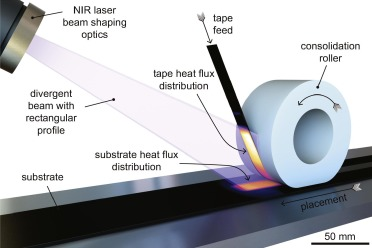
\includegraphics[width=0.6\textwidth]{img/afp_atl_machine.jpg}
	\caption{Draft of the functioning of an AFP/ATL machine.}
	\label{fig:afp-atl_machine}
\end{figure}

The head of the machine is fed from the fiber feeding system. A laser beam hits the contact area between the fed tape and the substrate (the laminates which are already placed). This slightly heats up the pre-impregnated resin to tack the material into place before undergoing the curing process at higher temperature and pressure. There is also a consolidation roller that applies pressure to ease and ensure the tape placement. Once the tape is placed, a cutter would cut the material to let the head to displace and re-start again the process.

These machines are controlled by numeric control programs allowing to control sever parameters of the process, such as the tape lying speed, compaction force or the heat source temperature[2].

In some cases, the mold is in a fixed position and the head of the machine moves near to the surface to place the material. In order to produce huge components, the head can be also attached to a rail that allows it to move faster to different points of the part.

There are even more complex machines in which both the head and the tool are moving perfectly synchronized. It is the case of the AIRBUS A350 tail cone (Section 19): the mold spins while the head is placing the plies of composite on it.

**FOTO**

\subsection{Autoclave}

Once the pre-shape is completed, the polymeric matrix must be cured. In order to achieve the optimum conditions, the part has to undergo at least one autoclave cycle, which basically is an oven that applies both temperature and pressure. For that, the material has to be carefully prepared with these elements:
\begin{itemize}
\item A \textbf{release film} to protect the composite. This also allows to remove the other materials placed above the prepreg component.
\item \textbf{Breather} and \textbf{bleeder} weave which fulfils two essential functions:
\begin{itemize}
\item Absorb the excess of resin that comes up while the prepreg is heated and exposed to a high pressure.
\item Let the gases stuck inside the material to get out, preventing the formation of voids inside of the material that could result in an important degradation of the mechanical properties of the final component.
\end{itemize}
\item \textbf{Vacuum bag} to cover the part and apply vacuum to it.
\item \textbf{Sealant tape} to seal the vacuum bag to the mold.
\item \textbf{Vacuum system} to create vacuum inside the bag.
\end{itemize}

**FOTO**

Once everything is prepared, the whole system is introduced into the autoclave and its door is closed. The autoclave starts rising its \textbf{temperature}, which is distributed along the interior by convection, and \textbf{pressure}, generally using an inert gas such as nitrogen.

The autoclave carries out a temperature and pressure cycle. It depends essentially on the thermoset resin to be cured and its curing characteristics. Also the geometrical features of the part such as thickness or shape have an influence. It is mandatory to control and ensure that 3 main parameters are within the specified limits (usually stablished by the R\&D departments of each company): heating rate during the ramp-up, cooling rate and the time of dwell within the established temperatures range[3]:

\begin{itemize}
\item \textbf{Temperature ramp-up}. The ramp-up ratio must be controlled and maintained inside the limits to avoid fast heating that could degrade the material and also too slow ratios that could lead to an incomplete curing reaction. Also the resin starts flowing becoming more homogenous and conforming a continuous interface to the fibers.
\item \textbf{Temperature stabilization} (or \textbf{dwell}). Here is where the curing reaction takes place. The dwell has to keep certain temperature (usually between 120 °C and 180 °C) within an error interval of ±5 °C to allow a correct curing reaction, while keeping adequate values of \textbf{pressure} and \textbf{vacuum} to assist the consolidation of the component and suppress the potential voids that could be formed due to air bubbles that could remain inside the matrix.
\item \textbf{Cooling down}. Its cooling rate must be also monitored and controlled within stablished limits to avoid fast cooling that could produce undesired internal stresses inside the material.
\end{itemize}

The autoclave cycle shown in the next figure has two ramp-ups, two stabilizations and the final cool down.

**FOTO**

\subsection{Final operations}

Once the component is cured, the prepreg material has already achieved its optimum mechanical properties. It is now prepared to undergo the final operastions that will give it its final shape:

\begin{itemize}
\item \textbf{Trimming} to achieve the final shape at the boundaries. During this process the prepregs are sensitive to suffer delamination. In the aerospace industry it is quite common to use energetic trimming methods to minimize this problem, such as Abrasive Water Jet (AWJ)[4], in which a high pressure water jet mixed with an abrasive material is ejected from a pistol with high pressure.
\item \textbf{Cleaning the part}. This process can be automated also, but the water pressure must be carefully adjusted to avoid delamination. Another option is manual cleaning, but it is a slower method.
\item \textbf{Non Destructive Testing (NDT)}. In the case of prepregs, the most suitable technique is the Ultrasonic Testing (UT). For huge components it is used an automated method (AUT), even though the manual testing can also be used in specific areas where an automated method cannot get to. The AUT methods use mechanized means to drive ultrasonic scanning equipment through the component being tested, saving more time. As it is known, the UT works with a transducer that generates high frequency ultrasonic energy, which is introduced and propagated through the material. If it detects a discontinuity, part of the energy will be reflected, detected and displayed on a screen. Typical equipment consists of a pulser/receiver, transducer and display units.
\item \textbf{Surface treatments} to prepare the component for a final bonding or painting, such as degreasing, abrasion, chemical cleaning or gas treatments.
\end{itemize}


\section{Fields of applications of prepreg materials}

\subsection{Space applications}

\section{Aeronautical applications}

The aeronautical industry is starting to introduce the use of composite materials
and reinforced plastic. During the past 20 years its use has become widely extended
in the manufacture of aircrafts and nowadays lot of parts of them are made by composites.
This sector is, every year, demanding more composites in order to meet its needs
to reduce weight, save costs and improve manufacturing times. The composite industries
is developing new methods to satisfy this needs, and many of these are based on
out-of-autoclave processes. These are faster than the traditional ones, allowing
big savings in operational costs. Some analysts are projecting that in the next
5 years there will be an increase in the global composite market for aerospace
applications of  33\% giving a total production of 43.5 million kg. \cite{2}

Another way to see the change in the aerospace industry, which is continuously
moving to composite material solutions, is analyzing the materials in which are
manufactured a series of commercial aircraft, for example, in the figure [2] is
shown the Boeing famous airplanes, where it can be observed a clear trend to use
more composites in the last decades\cite{3}.
[3] Xuesong Zhang, Yongjun Chen, Junling Hu. Recent advantages in development in aerospace materials

\begin{figure}[h]
	\centering
	\includegraphics[width=0.8\textwidth]{img/boeing_aircrafts.png}
	\caption[Carbon fiber prepreg roll]{Evolution of the
	series of Boeing commercial aircrafts in terms of the materials used in
	its manufacture, showing a clear increase in composite materials solutions
	in the lasts models, specially in the last Boeing 787. \cite{3}}
	\label{fig:prepreg_roll}
\end{figure}

\section{Conclusions}

Definitely, the introduction of pre-impregnated composites has supposed a
revolution within the aerospace industry. Despite the high cost of the tools,
machinery and processing, other features of this material such as the excellent
mechanical properties achieved, the fuel saving that allows and the relatively
easy automatization of the manufacturing processes, make prepregs a material for
the present and the future in the aerospace industry.\\

The incoming improvements will be focused in different aspects:\\

\begin{itemize}
	\item The increase in the automatization level of the processes and the
	speed and acceleration of the placement machines.
	\item New generation of prepregs Out of Autoclave (OoA).
\end{itemize}

Regarding the first point, the automated lying and fibre placement still have
certain manual tasks. Sometimes the laminates are not cut properly and get stuck in
the machine, or even the cutter can break, so the operators have to stop the process
and fix this problem manually. Also changing the roll of material when the machine
has run out of it has to be done manually. The aim is to get rid of as most manual
tasks as possible in order to decrease the process time. Another approach is to
increase the fibre placement velocity to allow a higher weight of placed material
per minute.\\

Concerning the prepregs OoA, it is clear that an autoclave cycle is an
expensive task due to its huge energy consumption. For some components, such as
the AIRBUS A350 wing lower cover, an autoclave cycle can last up to 10 hours.
Some studies have been carried
out in order to develop a new generation of prepregs that only need a conventional
oven to be cured, without the presence of high pressure to compact the plies.
Good results have been
obtained so far for parts with thickness less than 2mm, achieving microstructural,
thermal and mechanical properties very similar to components cured in autoclave.\\
